\documentclass[12pt,oneside]{book}
\usepackage{geometry}                		% See geometry.pdf to learn the layout options. There are lots.
\geometry{a4paper}                   			% ... or a4paper or a5paper or ... 
%\geometry{landscape}                		% Activate for for rotated page geometry
%\usepackage[parfill]{parskip}    		% Activate to begin paragraphs with an empty line rather than an indent
\usepackage{graphicx}				% Use pdf, png, jpg, or epsß with pdflatex; use eps in DVI mode
								% TeX will automatically convert eps --> pdf in pdflatex		
\usepackage{amssymb}

\usepackage[spanish]{babel}			% Permite que partes automáticas del documento aparezcan en castellano.
\usepackage[utf8]{inputenc}			% Permite escribir tildes y otros caracteres directamente en el .tex
\usepackage[T1]{fontenc}				% Asegura que el documento resultante use caracteres de una fuente apropiada.

\usepackage{hyperref}				% Permite poner urls y links dentro del documento

\title{Manual de Juego Sudoku}
\author{Manuel Suárez-Veronica Pozo-José Salas}
%\date{}							% Activate to display a given date or no date

\begin{document}
\maketitle
\tableofcontents

\chapter{Introducción}

El libro a continuación es creado para demostrar el proyecto realizado, Sudoku. 
En el cual se utilizara el lenguaje c++ (Orientado a objetos) para programarlo, utilizaremos la libreria "Qt" y una interfaz gráfica para el desarrollo del mismo llamado
"Qt Creator". 
	\includegraphics[width=0.8\textwidth]{./imagenes/qt.png}

\chapter{El Juego}
	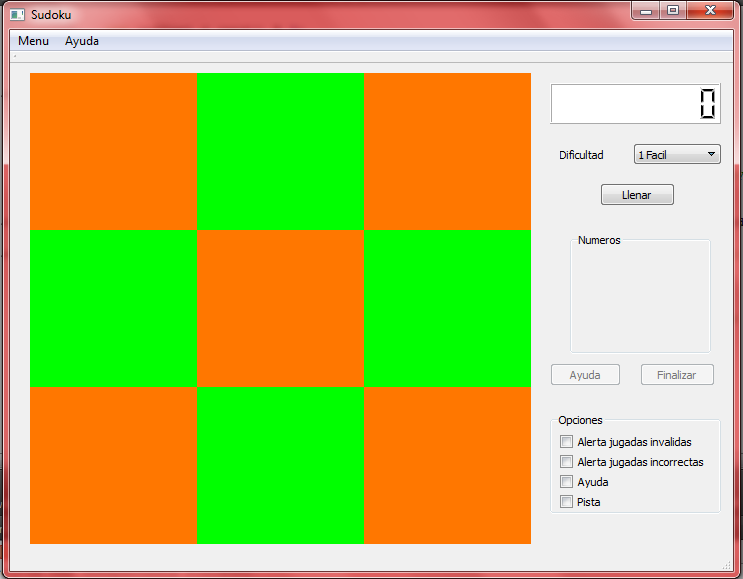
\includegraphics[width=0.8\textwidth]{./imagenes/PantallaPrincipal.png}
	Sudoku es un pasatiempo que se publicó por primera vez a finales de la década de 1970 y se popularizó en Japón en 1986, dándose a 
	en el ámbito internacional en 2005 cuando numerosos periódicos empezaron a publicarlo en su sección de pasatiempos. 1 El objetivo del sudoku es rellenar una cuadrícula de 9 × 9 celdas 
	dividida en subcuadrículas de 3 × 3 (también llamadas "cajas" o "regiones") con las cifras del 1 al 9 partiendo de algunos números ya dispuestos en algunas de las celdas. 
	Aunque se podrían usar colores, letras, figuras, se conviene en usar números para mayor claridad, lo que importa, es que sean nueve elementos diferenciados, que no se deben repetir en una misma fila,
	columna o subcuadrícula. Un sudoku está bien planteado si la solución es única. La solución de un sudoku siempre es un cuadrado latino, aunque el recíproco
	en general no es cierto ya que el sudoku establece la restricción añadida de que no se puede repetir un mismo número en una región.

\chapter{Historia}
El Sudoku puede haberse ideado a partir de los trabajos del matemático suizo Leonhard Euler (1707-1783), quién utilizó los cuadrados latinos1 para realizar cálculos probabilísticos,
aunque su aparición más obvia se dio en el año 1979, cuando el norteamericano Howard Garns publica en Nueva York, a través de la empresa Dell Magazines, un juego muy similar conocido
bajo el nombre de “Number Place”. En el año 1984 una editorial japonesa lo exportó hacia ese país, divulgándolo en el periódico “Monthly Nikolist” bajo el nombre de “Los números deben estar solos” 
(cuyo apócope en japonés es SuDoku). La editorial introdujo con el correr de los años algunas innovaciones que hicieron que el juego ganara gran popularidad entre los lectores. 
Sus inicios reales como Sudoku en Occidente se remontan a los años 2004/2005, gracias a su publicación en los diarios “The Times” y “The Daily Mail”. Desde aquel entonces,
el juego ha alcanzado una gran popularidad en el mundo moderno: en 2005 se publicó el primer libro acerca de Sudokus en el mundo (“Los mejores Sudokus”, con 200 tableros agrupados en 4 niveles de dificultad)
y se lo incluyó entre los 9 problemas del ICPC (sigla de International Collegiate Programming Contest). 
\chapter{Aplicación}
	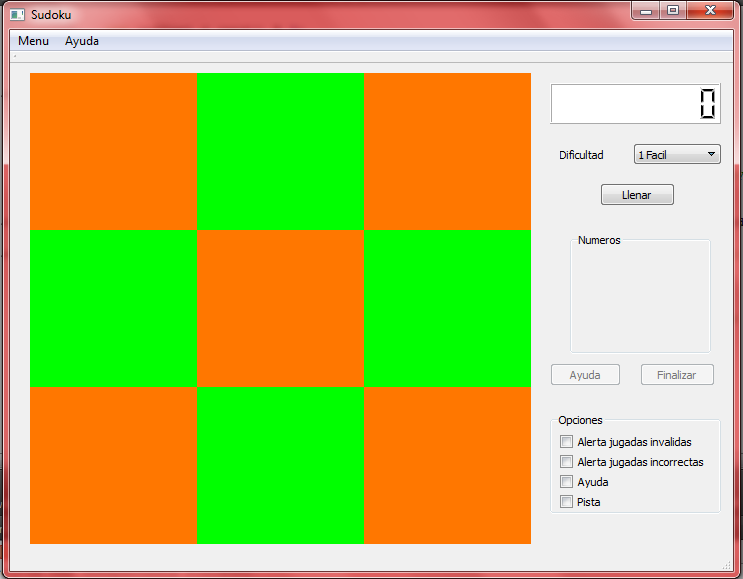
\includegraphics[width=0.8\textwidth]{./imagenes/PantallaPrincipal.png}
	Nuestra aplicación tiene una ventana principal donde podemos apreciar un menu bar con dos opciones:
		\begin{itemize}
			\item Menu 
			Nos da las opciones de cargar y guardar partica, ademas de salir del programa.
			\item Ayuda
			Nos da las opciones de Ayuda para el programa y y un acerca de.
			\end {itemize}
	Tenemos en el panel izquierdo:
	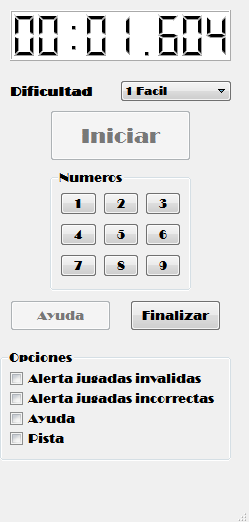
\includegraphics[width=0.8\textwidth]{./imagenes/Panel_izquierdo.png}
		\begin{itemize}
			\item LCD
			Widget LCD para mostrar el tiempo. 
			\item ComboBox
			Widget para elegir el nivel de dificultad.
			\item Boton
			Boton para generar y mostrar el tablero de Sudoku.
			\item Matriz 3x3 de Botones
			Botones para poder llenar el tablero
			\item Boton
			Boton de ayuda y Finalizar juego. (Ayuda se activa con los checkbox de abajo)
			\item CheckBox
			Conjunto de Checkbox para activar las alertas de jugadas inválidas,incorrectas,Ayuda,Pista.
			\end {itemize}
	
	Las matrices 3x3 que componen el tablero 9x9 se aprecian así:
	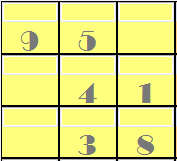
\includegraphics[width=0.8\textwidth]{./imagenes/cuadr9x9.png}
	La casilla hereda de QFrame con un QLineEdit y un Boton, y con el Qframe se puso fondo. 
	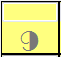
\includegraphics[width=0.8\textwidth]{./imagenes/Casilla.png}
	Una jugada Invalidad y una jugada incorrecta se muestra asi:
	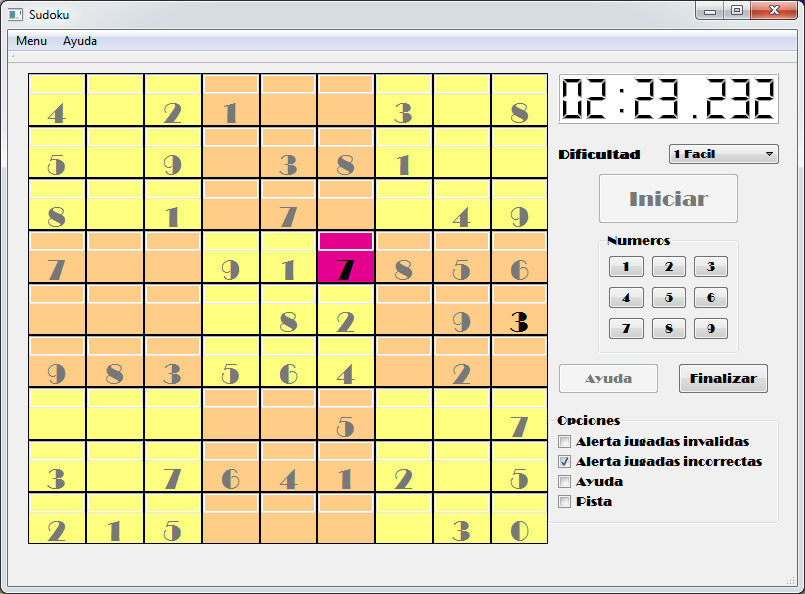
\includegraphics[width=0.8\textwidth]{./imagenes/jugada_incorrecta.png}
	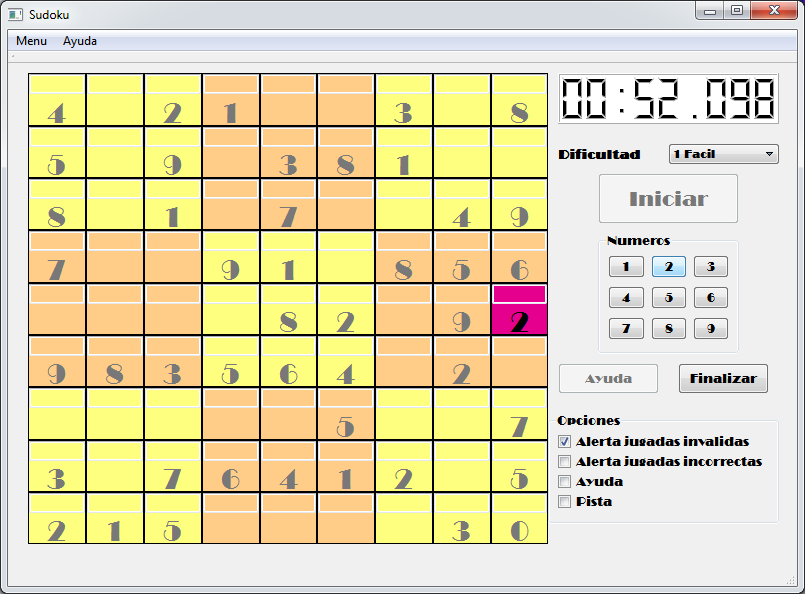
\includegraphics[width=0.8\textwidth]{./imagenes/jugada_invalida.png}
	La opción pista nos da un numero random correcto, y se muestra así:
	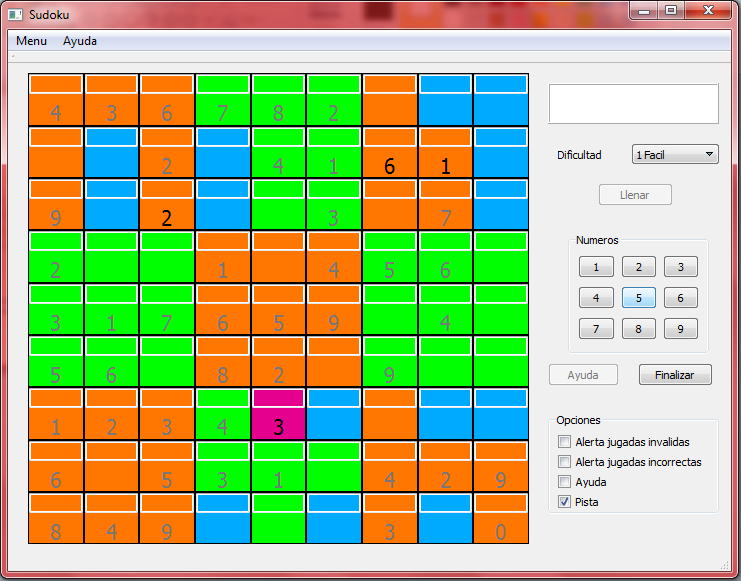
\includegraphics[width=0.8\textwidth]{./imagenes/pista_juego.png}  
	
	
\chapter{Funcionalidad}
\begin{center} Generacion de tableros:\end{center}
\begin{itemize}
\item  Algoritmo implementado.
\begin{itemize}
	\item Se genera un tablero con numeros random hasta que este sea resolvible.
	\item Se verifica si es resolvible.
	\item Se trata de resolver por arreglos de posibildades de numeros en casillas.
	\item Si no se puede resolver así, se utiliza la técnica del Backtracking. 
	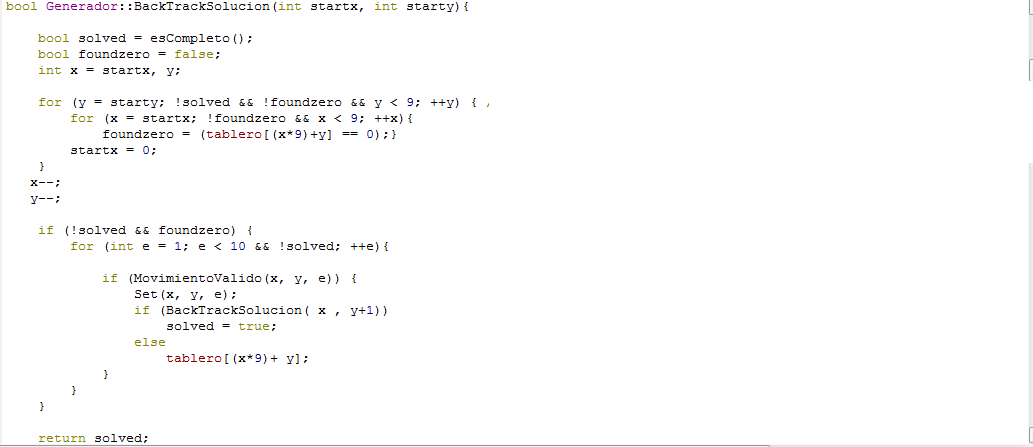
\includegraphics[width=0.8\textwidth]{./imagenes/Codigo_backtrcking.png}
	\item Utizando Backtracking se busca solucionar cambiando los numeros detras del vacio, y utilizando recursion de la misma.
	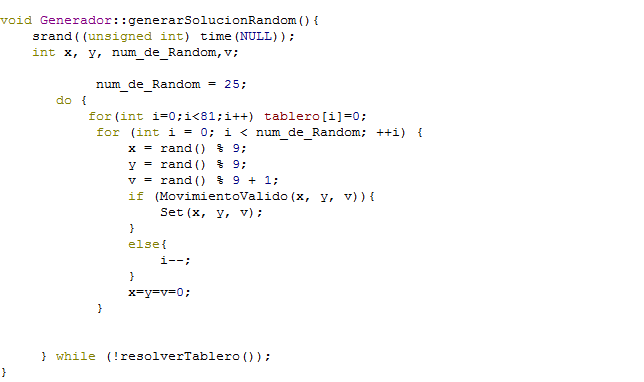
\includegraphics[width=0.8\textwidth]{./imagenes/codigo_genrador.png}
	jugada_incorrecta.png
	jugada_invalida.png
	pista_juego.png
\end {itemize}

\item  Dificultad.
\begin {itemize}
	\item Se procede a quitar numeros del arreglo, y comprobar si se puede resolver y tienen única solución.
	\item Se agregan en un pila los numeros y posiciones que fueron quitadas y se podia obtener única solución.
	\item Segun el numero de dificultad se obtienen posiciones random repetidamente tantas casillas hay, y se ve las veces 
	que puede estar ese numero.


	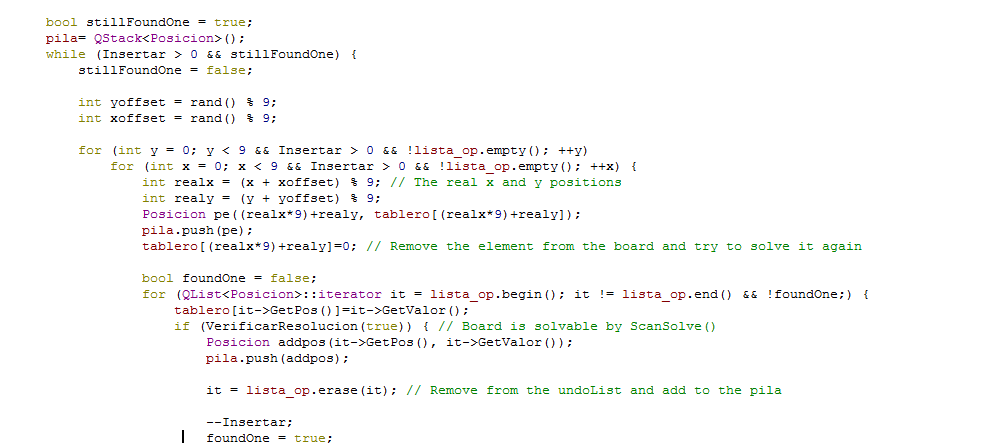
\includegraphics[width=0.8\textwidth]{./imagenes/Codigo_dificultad.png}
\end {itemize}
\item  Guardar y cargar tableros cifrados .

	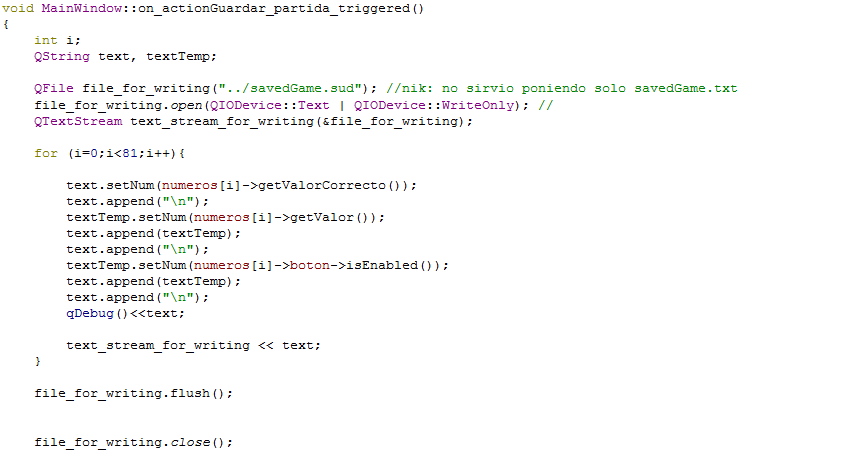
\includegraphics[width=0.8\textwidth]{./imagenes/Codigo_archivo_guardar.png }		
\item   Jugar y finalizar juego (2).
 	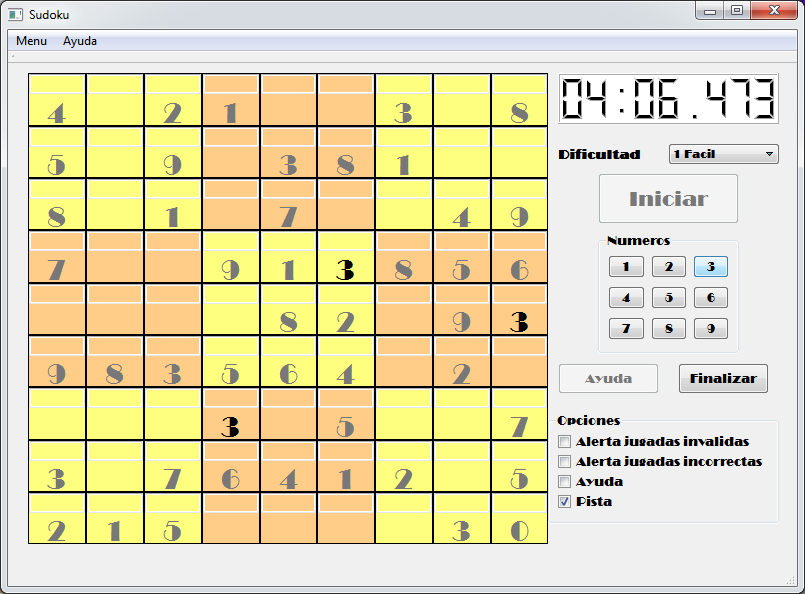
\includegraphics[width=0.8\textwidth]{./imagenes/PantallaJugando.png}
	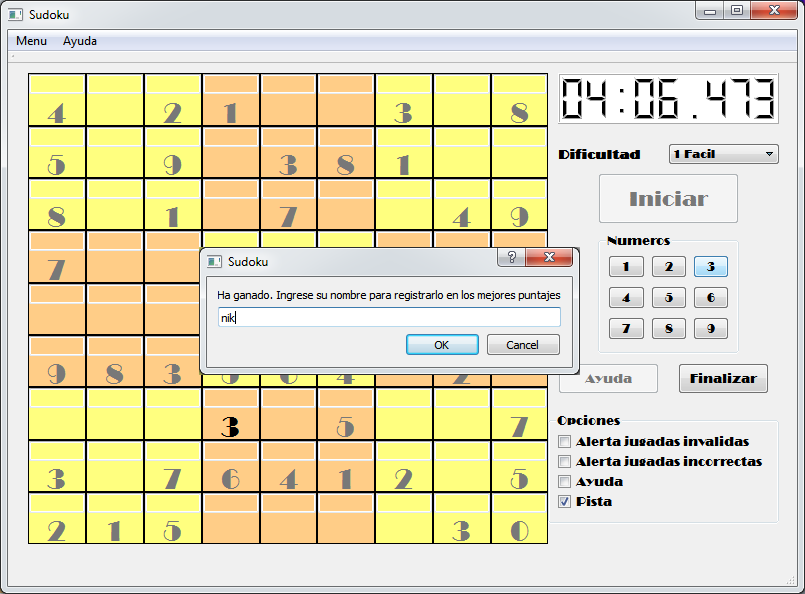
\includegraphics[width=0.8\textwidth]{./imagenes/Codigo_finalizar.png}
\item   Puntaje (3).
	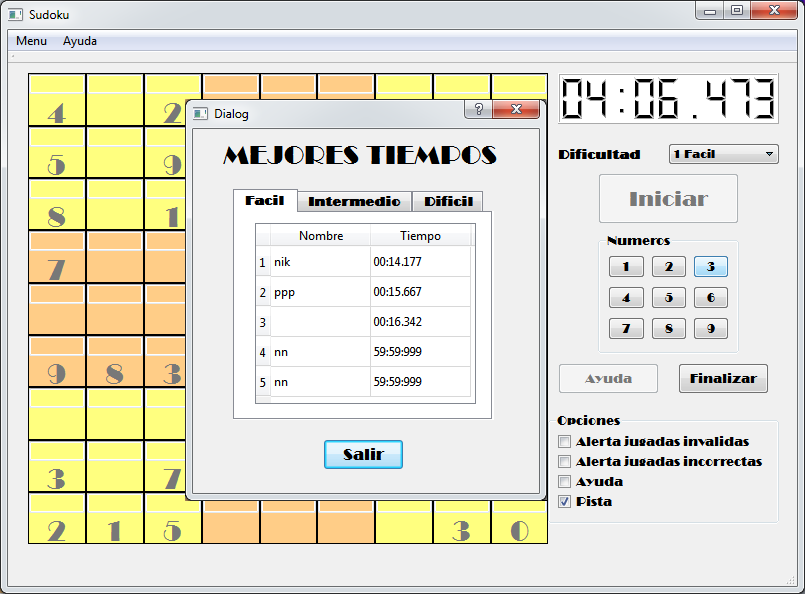
\includegraphics[width=1.10\textwidth]{./imagenes/puntaje.png}
\end{itemize}

\chapter{Colaboraciones}

\begin {itemize}	

\item Commits por integrante.
\begin{itemize}
\item Veronica Pozo: 18
\item Manuel Suárez: 19
\end
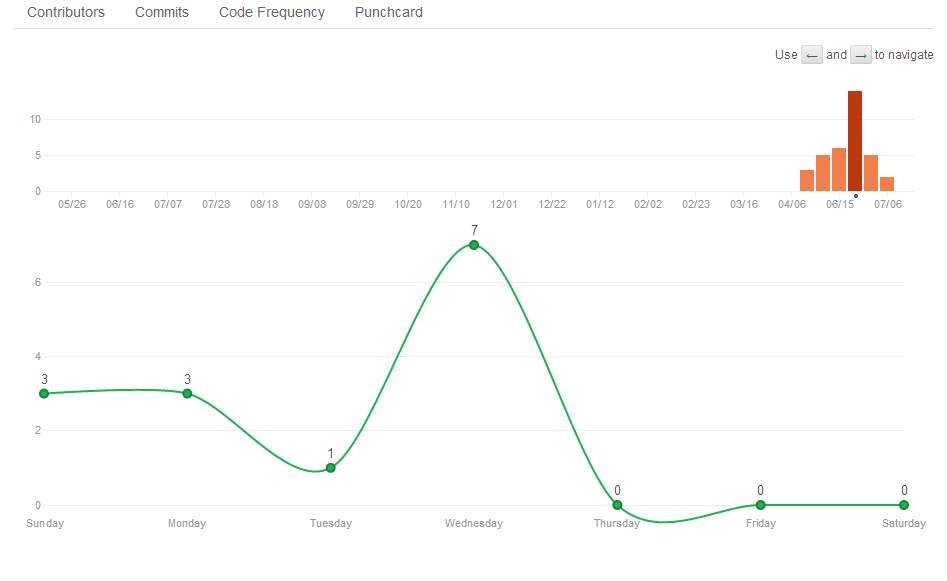
\includegraphics[width=1.10\textwidth]{./imagenes/Contribuidores_commit_linea.png}
\item ¿En qué fechas hay picos?
\begin{itemize}
\item 14 de Junio
\item 3 de Julio
\end
	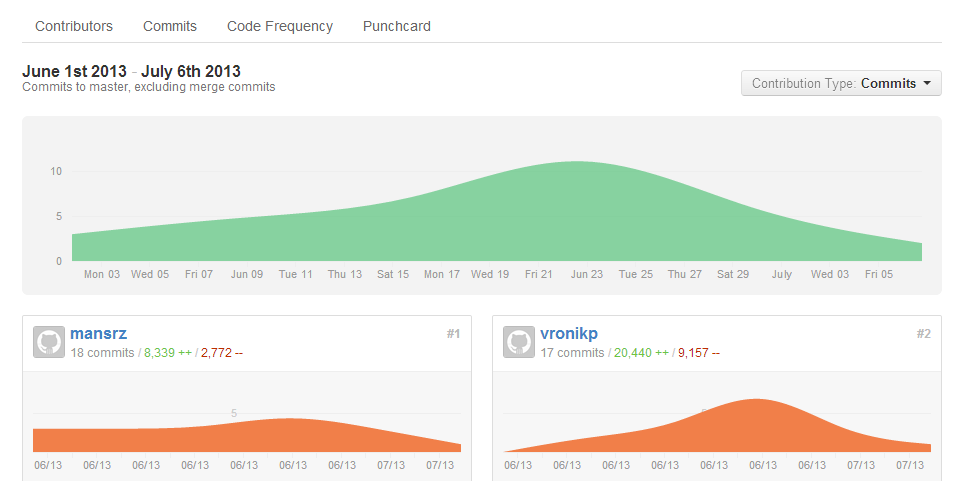
\includegraphics[width=1.10\textwidth]{./imagenes/Contribuidores_commit.png}
\end{itemize}
\chapter{Conclusiones}
Se concluye
\end{document}  
